\chapter{Opis stworzonego rozwiązania}
\label{cha:rozwiazanie}

Niniejszy rozdział zawiera opis systemu, który został stworzony na potrzeby tej pracy. W rozdziale~\ref{sec:zalozeniaProjektowe} zostały krótko przedstawione najważniejsze założenia, na których opiera się realizacja projektu. Następnie rozdział~\ref{sec:architekturaSystemu} opisuje architekturę stworzonego rozwiązania. Rozdział~\ref{sec:modelDanych} zawiera szczegółowy opis w jaki sposób został określony model danych. Sposób działania algorytmu grupowania został zaprezentowany w rozdziale~\ref{sec:gruperNFZ}. Spojrzenie na system z punktu widzenia systemu ekspertowego został zawarty w sekcji~\ref{sec:systemEkspertowy}. Rozdział~\ref{sec:optymalizacjaJGP} przedstawia realizację maszyny wyjąśniającej, która jest narzędziem umożliwiającym przeprowadzenie optymalizacji JGP w systemie.

%---------------------------------------------------------------------------
%---------------------------------------------------------------------------
\section{Założenia projektowe}
\label{sec:zalozeniaProjektowe}

Na kształt aplikacji bezpośredni wpływ miały założenia projektowe postawione na początku pracy. Od nich zależały decyzje podejmowane na kolejnych etapach tworzenia systemu. Lista założeń projektowych przedstawia się następująco:

\begin{enumerate}
 \item Swtorzyć aplikację typu ,,Gruper'' spełniającą wszystkie wymagania stawiane przez NFZ.
 \item Określić model danych, ustalić bazę wiedzy.
 \item System zostanie napisany w języku JAVA, będzie to aplikacja desktopowa z dostępem do bazy wiedzy, zapisanej w jednym pliku.
 \item Zastosować architekturę warstwową.
 \item Użyć najnowszych i najlepszych narzędzi do tworzenia przyjaznego dla użytkownika GUI.
 \item Projekt architektury oprzeć na metodologii Spring.
 \item W trakcie fazy implementacji zwrócić szczególną uwagę na to, aby system spełniał założenia systemu ekspertowego. Implementacja systemu będzie zalążkiem do stworzenia bardziej rozbudowanego systemu ekspertowego dla tego rozwiązania.
 \item Używać tylko narzędzi dostępnych na licencji wolnego oprogramowania.
 \item Wykonać testy dla wszystkich głównych ścieżek poszukiwań rozwiązania.
\end{enumerate}

Stworzenie aplikacji typu ,,Gruper'' oznacza, że musi zostać zaimplementowany algorytm ,,Grupera'' zgodnie z wytycznymi narzuconymi przez NFZ. Precyzyjne określenie modelu danych jest podstawowym założeniem, bez którego niemożliwa jest dalsza praca nad projektem. Zastosowanie architektury warstwowej dla systemu zwiększa elastyczność rozwiązania i pozwala na łatwe modyfikowanie i skalowalność systemu.

Implementacja całego systemu tylko w języku JAVA umożliwia rozwijanie projektu przez osoby nie znające składni oraz zasad jakimi kierują się inne języki dedykowane dla systemów ekspertowych takie jak Prolog czy Drools. Wszystkie założenia systemu ekspertowego zostają spełnione, a implementacja będzie w 100\% autorska. Fakty i reguły będą obiektami JAVY. Unikalność, innowacyjność i łatwość wdrożenia się w projekt dla tego rozwiązania mają być jego największymi atutami.



%---------------------------------------------------------------------------
%---------------------------------------------------------------------------
\section{Architektura systemu}
\label{sec:architekturaSystemu}

Wybór architektury systemu to decyzja podejmowana w początkowej fazie tworzenia systemu. Często okazuję się ona najważniejszą decyzją, która ma ogromny wpływ na rozwój oprogramowania\cite{sienkiewicz_architektura}. Kierując się wyborem architektury postawiono na jej elastyczność oraz modularność. Obrazując system jako maszynę złożoną z wielu rożnorodnych elementów dążono do stworzenia takiej, którą można w łatwy sposób ulepszać poprzez dokładanie nowych klocków oraz naprawiać poprzez podmianę starych części nowymi i lepszymi.

%---------------------------------------------------------------------------
\subsection{Model warstwowy}
\label{sec:model3warstwowy}
Architektura systemu odzwierciedla jego logiczny podział. Standardem w praktycznie każdej aplikacji jest zastosowanie modelu architektury warstwowej\cite{sienkiewicz_architektura}. Model wprowadza podział aplikacji na trzy warstwy:
\begin{enumerate}
 \item \textbf{Warstwę danych} odpowiedzialną za poprawne przechowywanie, zapis oraz odczyt danych.
 \item \textbf{Warstwę logiki biznesowej}, której zadaniem jest koordynacja pracy aplikacji, przetwarzanie żądań użytkownika, aplikacja reguł logicznych, dokonywanie obliczeń.
 \item \textbf{Warstwa prezentacji} wykonująca tłumaczenie żądań i wyników działania aplikacji do i z języka zrozumiałego dla użytkownika.
\end{enumerate}

Wybrano ten model do zastosowania przy tworzeniu aplikacji ze względu na jego logiczną i zrozumiałą dla każdego informatyka modularność. Każda z warstw może zostać zaimplementowana w innym języku programowania, a komunikują się one poprzez interfejsy. Dużym plusem tego rozwiązania jest łatwa możliwość zmiany pewnej części systemu bez zmian w innych częściach systemu. Dla przykładu, jeśli zaszłaby potrzeba stworzenia webowego interfejsu użytkownika to wystraczy tylko zaimplementować warstwę prezentacji i podpiąć ją do warstwy logiki biznesowej.

Architekturę trójwarstwową przedstawia rysunek \ref{img:rysunek_3layer}.
\begin{figure}[!ht]
\centering	
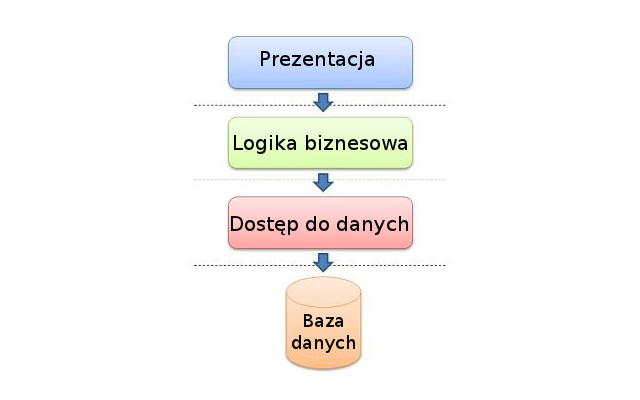
\includegraphics[scale=0.5]{images/3layer-architect}
\caption[Rysunek przedstawiający model architektury trójwarstwowej]{Architektura trójwarstwowa. Autor: Mateusz Urbanik}
\label{img:rysunek_3layer}
\end{figure}

%---------------------------------------------------------------------------
\subsection{Środowisko Spring}
\label{sec:modelArchitekturySpring}
Bardzo popularnym i nowoczesnym środowiskiem, które wprowadza zestaw narzędzi, wzorców oraz bibliotek potrzebnych do stworzenia nowoczesnych aplikacji serwerowych(i nie tylko) jest Spring. Rozwiązanie to jest niesłusznie uważane za skomplikowane, bardzo złożone i niemożliwe do opanowania. W rzeczywistości Spring stanowi zaawansowany przykład architektury szkieletowej umożliwiającej szybkie rozwijanie dowolnie złożonych aplikacji, niekoniecznie webowych. Konstrukcja szkieletu architektury Spring powoduje, że występuje w nim bardzo niewielki stopień zależności od interfejsów Spring API. Architektura Spring obejmuje wszystkie warstwy aplikacji i podsuwa rozwiązania, które mogą być stosowane zarówno w warstwie prezentacji, jak i w warstwie integracji oraz warstwie danych. Szkielet aplikacyjny Spring jest rozwijany na licencji ,,open source'' od roku 2003 i od tego czasu zdobył sobie dużą popularność\cite{bruce_spring}. Rysunek \ref{img:rysunek_spring} ilustruje schemat architektury Spring.

\vspace*{0.1cm}
\begin{figure}[!ht]
\centering
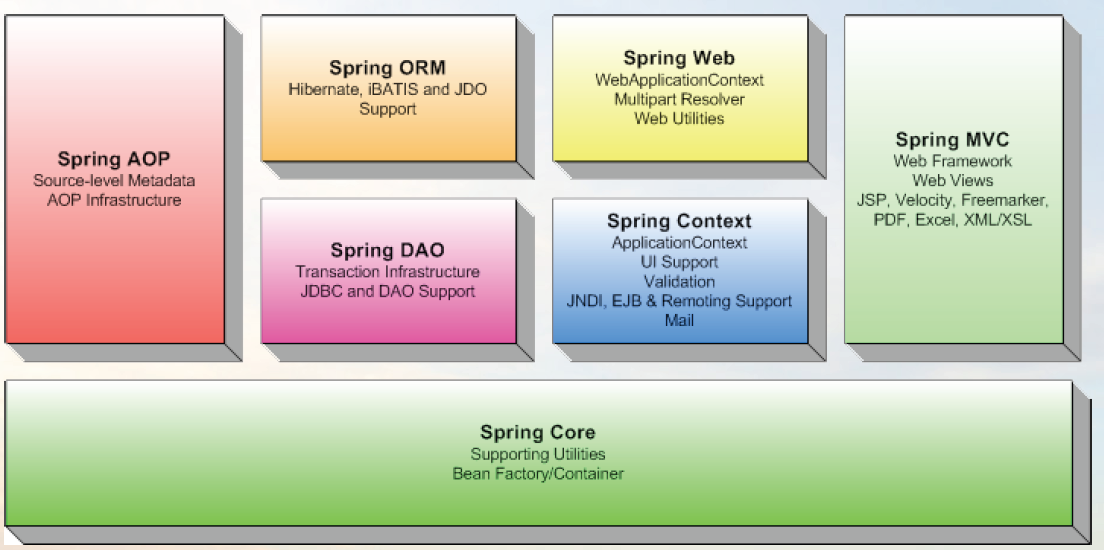
\includegraphics[scale=0.31]{images/spring-modules}
\caption[Rysunek przedstawiający model architektury Spring]{Schemat architektury Spring. Źródło: Spring Reference Guide\cite{spring_reference}}
\label{img:rysunek_spring}
\end{figure}

Spring składa się z kilku modułów, z których każdy może być niezależnie używany w aplikacji. Oznacza to, że aplikacja może wykorzystywać wszystkie możliwości środowiska Spring, ale może także korzystać z fragmentu architektury, np. z modułu ułatwiającego dostęp do danych. Najważniejszym modułem jest Spring-Core. Jest to moduł oferujący zaawansowane opcje konfiguracji komponentów JavaBean oraz klas POJO(ang. Plain Old Java Object) i wykorzystujący technikę wstrzykiwania zależności.
W aplikacji postanowiono wykorzystać kilka bazowych elementów architektury. Oto lista modułów Spring wykorzystywanych w projekcie:
\begin{itemize}
 \item JDBC - Java DataBase Connectivity - interfejs programowania opracowany w 1996 r. przez Sun Microsystems, umożliwiający niezależnym od platformy aplikacjom napisanym w języku Java porozumiewać się z bazami danych za pomocą języka SQL.
 \item DAO(ang. Data Access Object) - wzorzec projektowy wprowadzający rozdzielenie mechanizmu trwałości obiektów od reguł biznesowych.
 \item Service - Spring Service Beans - obiekty serwisowe wykonujące logikę biznesową.
\end{itemize}

Dla warstwy prezentacji wykorzystałem również wsparcie Spring. W 2008 roku została wydana przez społeczność Spring pierwsza wersja środowiska do tworzenia aplikacji desktopowych w JAVIE - SpringRCP - Rich Client Project. Niestety po wydaniu wersji 1.1 w 2009 roku projekt, który był na wyższym technologicznie poziomie niż NetBeans-RCP lub Eclipse-RCP z nieznanych powodów przestał być rozwijany\cite{spring_rcp_reference}. W roku 2011 jeden z głównych projektantów Spring-RCP postanowił go odświeżyć. W niecałe 6 miesięcy przepisano całe środowisko używając najnowszej metodologii pochodzącej z Spring 3. Nowa wersja projektu otrzymała nazwę Valkyrie-RCP\cite{valkyrie_reference}. W kolejnych iteracjach dodanych zostało wiele nowych funkcjonalności, w wyniku których po kolejnych 3 miesiącach powstało solidne narzędzie do tworzenia skomplikowanych aplikacji desktopowych w JAVIE. Jego podstawowe cechy to przejrzystość, prostota, stosowanie dobrych wzorców GUI.
Podstawowe elementy pakietu Valyrie-RCP, które wykorzystano do stworzenia aplikacji to\cite{valkyrie_reference}:
\begin{itemize}
 \item Widget - komponent GUI (tabelka, forma, widok, edytor-danych).
 \item DataProvider - fasada danych dla komponentów UI.
\end{itemize}

Rysunek \ref{img:rysunek_spring2} przedstawia architekturę systemu jaki został zaimplementowany.

\begin{figure}[!ht]
\centering
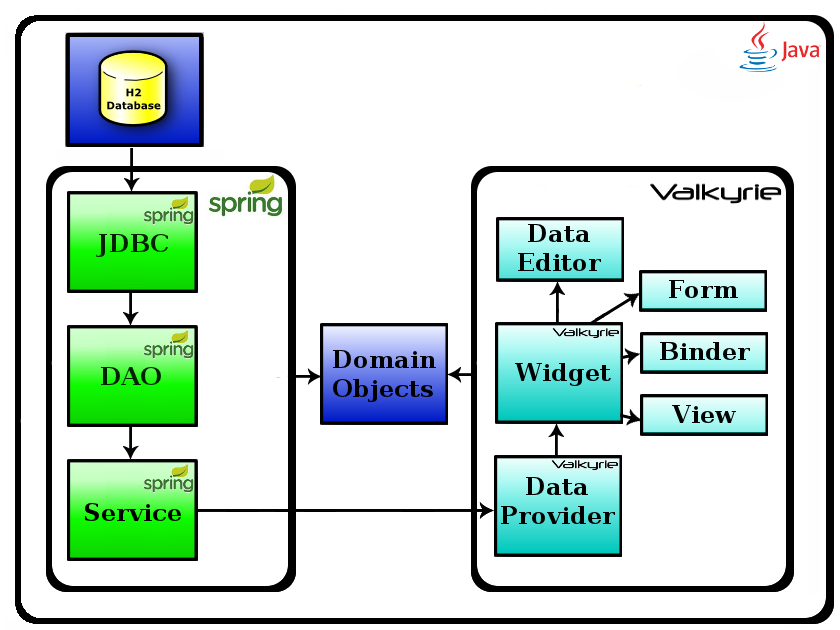
\includegraphics[scale=0.4]{images/spring-layers2}
\caption[Rysunek przedstawiający model architektury systemu]{Architektura systemu stworzonego dla pracy. Autor: Mateusz Urbanik}
\label{img:rysunek_spring2}
\end{figure}

Należy zaznaczyć, że model architektury spełnia założenia architekty trójwarstwowej:
\begin{table}[h]
 \caption{Moduły Spring jako elementy architektury trójwarstwowej}
 \small\tt
 \centering
 \vspace{0in}
 \begin{tabular}{|l|l|}
 \hline
 \textbf{Element architektury 3-warstwowej} & \textbf{Moduły systemu} \\ 
 \hline
 Dostęp do danych & H2-Database, JDBC, DAO \\
 \hline
 Logika biznesowa & Services \\
 \hline
 Prezentacja & Valkyrie-RCP \\
 \hline
 \end{tabular}
\end{table}

%---------------------------------------------------------------------------
\subsection{Architektura systemu ekspertowego}
\label{sec:architekturaSystemuEkspertowego}
Jedna z definicji systemu ekspertowego definiuje go jako system charakteryzujący się strukturą\cite{goluchowski_eskpertowe}:
\begin{itemize}
 \item 	Szkielet,
       \begin{itemize}
	 \item Interfejs użytkownika,
	 \item Edytor bazy wiedzy,
	 \item Systemu wnioskujący,
	 \item Mechanizm wyjaśniający,
       \end{itemize}
 \item Baza wiedzy,
 \item Dynamiczna baza danych.
\end{itemize}

Bardzo istotnym elementem systemu ekspertowego jest oddzielenie wiedzy dziedzinowej od reszty systemu. Takie podejście umożliwia usprawnienie działania systemu bez ingerencji w kod programu. W~skrócie wyjaśnię elementy architektury systemu ekspertowego.

\textbf{Interfejs użytkownika} umożliwia zadawanie pytań, udzielanie informacji systemowi oraz odbieranie od systemu odpowiedzi i wyjaśnień.
\textbf{Edytor bazy wiedzy} pozwala na modyfikację wiedzy zawartej w systemie, umożliwiając tym samym jego rozbudowę.
\textbf{Mechanizm wnioskowania} jest głównym składnikiem systemu ekspertowego wykonującym cały proces rozumowania w trakcie rozwiązywania problemu postawionego przez użytkownika.
\textbf{Mechanizm wyjaśniający} jest to jeden z elementów interfejsu pomiędzy systemem a użytkownikiem, który umożliwia użytkownikowi uzyskanie odpowiedzi dlaczego system udzielił takiej, a nie innej odpowiedzi, albo dlaczego system zadał użytkownikowi określone pytanie.
\textbf{Baza wiedzy} jest to deklaratywna postać wiedzy ekspertów z danej dziedziny zapisana za pomocą wybranego sposobu reprezentacji wiedzy, najczęściej reguł.
\textbf{Dynamiczna baza danych} jest pamięcią roboczą przechowującą pewne fakty wprowadzone w trakcie dialogu z użytkownikiem. Baza ta umożliwia odtworzenie sposobu wnioskowania systemu i przedstawienie go użytkownikowi za pomocą mechanizmu wyjaśniającego\cite{martyniuk_ekspertowe}.
Architekturę systemu regułowego przedstawia rysunek \ref{img:rysunek_expert}.
\begin{figure}[!ht]
\centering	
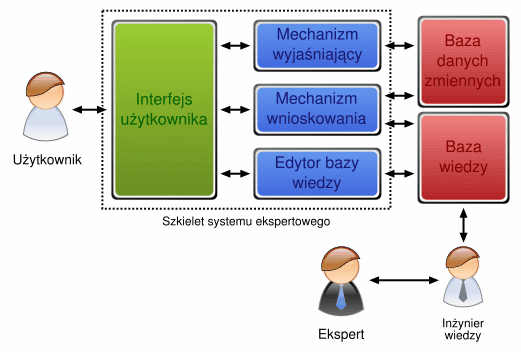
\includegraphics[scale=0.5]{images/expert-system}
\caption[Rysunek przedstawiający model architektury systemu ekspertowego]{Architektura systemu ekspertowego. Autor: Mateusz Urbanik}
\label{img:rysunek_expert}
\end{figure}

%---------------------------------------------------------------------------
\begin{comment}
\subsection{System ekpertowy w architekturze Spring}
\label{sec:systemEkpertowyArchitekturaSpring}

Na początku pracy postawiona została teza: realizacja systemu ekspertowego w architekturze spring spełniającego wymagania dotyczące aplikacji grupera oraz zawierającego optymalizację grupowania.

Popularne narzędzia do implementacji systemu ekspertowego to język Prolog, system Drools, Jess, CLIPS. Są to gotowe środowiska do budowania skomplikowanych systemów ekspertowych. Dla tych systemów wystarczy zdefiniować wiedzę w postaci faktów i reguł, a następnie zadać cele, aby otrzymać wynik. Nie zdecydowałem się jednak na użycie tych dedykowanych systemów z dwóch ważnych powodów. Po pierwsze w mojej pracy postanowiłem zrobić coś innowacyjnego, a mianowice chciałem zbudować swój autorski system ekspertowy od podstaw zarazem używając do jego budowy nowoczesnych narzędzi. Po drugie stworzenie chociaż zalążka takiego innowacyjnego systemu w najnowszej technologii będzie już sporym osiągnięciem. Spojrzenie na system ekspertowy z naciskiem na jego realizację w czystej JAVIE może przynieść ciekawe rezultaty. 

Ten sposób myślenia doprowadził mnie do punktu, w którym musiałem jasno określić, które elementy systemu ekspertowego będą zaimplementowane przez które elementy architektury Spring. I tak określiłem, że warunki dla spełnienia reguł mogą być zapisywane jako obiekty POJO w bazie danych. Same reguły mogą być zapisywane w bazie poprzez sygnatury metod do wykonania lub jako skrypty napisane w języku Groovy(obiektowy język skryptowy wzorowany na składni Javy). Dynamiczna baza wiedzy będzie zrealizowana za pomocą obiektów POJO zapisywanych w bazie danych. Interfejs użytkownika  powstanie przy użyciu środowiska ValkyrieRCP, oraz jego wzorca DataEditor, który umożliwi dodawanie, edycję, usuwanie a nawet filtrowanie faktów oraz uruchamianie algorytmu wnioskowania. System wnioskujący będzie zrealizowany w warstwie biznesowej/serwisowej, gdzie zostanie zaimplementowany mechanizm wnioskowania. Będzie on wybierał dla danych wejściowych zestaw reguł i warunków, następnie wywoła metody sprawdzające i wykona odpowiednie działania jeśli warunki są spełnione. Mechanizm wyjaśniający zaimplementowany zostanie również w warstwie biznesowej.
\end{comment}

%---------------------------------------------------------------------------
%---------------------------------------------------------------------------
\section{Model danych}
\label{sec:modelDanych}

W tym podrozdziale znajduje się opis w jaki sposób stworzony został model danych dla aplikacji.

%---------------------------------------------------------------------------
\subsection{Dane wejściowe NFZ}
\label{sec:daneWejscioweNFZ}
Jedynym źródłem danych wejściowych dla aplikacji były rozporządzenia NFZ opublikowane na oficjalnej witrynie internetowej Funduszu\cite{rozporzadzenia_nfz}. Fundusz opublikował ponad 30 wersji pliku parametryzującego w formacie MS-Excel. W pliku tym znajdują się arkusze kalkulacyjne, w których dane zostały zapisane w postaci tabel. Każda następna wersja pliku parametryzującego począwszy od wersji pierwszej dostarcza zaktualizowane dane(np. nowe kody rozponań, procedur). Z kolejnymi wydaniami pliku poprawione zostały drobne błędy związane z formatem zapisu danych. Aby zobrazować sposób w jaki dane zmieniały się przeanalizowano zapis w kolumnie ranga procedury. Ranga większa niż 2 była zapisywana początkowo jako napis '>2', zmieniono ten zapis na wartość '3'. Ze względu na fakt, iż wiele poprawiono wraz z wydaniami kolejnych wersji pliku parametryzującego postanowiono pracować na wersji 25, która jest jedną z najnowszych. 

Kolejne wersje pliku z danymi nie wnosiły żadnych zmian do modelu danych, który pozostawał dalej źle zdefiniowany. Dla przykładu arkusz o nazwie 'JPG' zawiera listę kodów JGP, gdzie jako wartości kolumn przyjęte zostały wartości oddziałów, a na przecięciu wiersza(kodu, kodu produktu, nazwy JGP) i kolumny(oddział) postawiony został krzyżyk(znak 'X'). Inny przykład źle zdefiniowanego modelu danych to arkusz, w którym zapisane są wartości punktowe dla kodów JGP. W arkuszu tym zostały przepisane jeszcze raz wszystkie kody JGP, kody produktu i nazwy grup, a obok podane zostały wartości punktowe. Jeszcze jednym przykładem nieprawidłowego zapisu danych jest zdefiniowanie w arkuszu 'procedury' redundantnych danych. Kody i nazwy procedur zostały zwielekrotnione, chociaż różniły się one jedynie kolumną 'typ listy'.

Plik parametryzujący dostarczał redundantne dane, zwielokrotnione wartości w wielu tabelach, nieokreślone zostały klucze podstawowe, obce, ani ograniczenia unikalności. Po wykonaniu dogłębnej analizy pliku wyciągnięto następujący wniosek: model danych dostarczany przez NFZ musi zostać przekonwertowany tak, aby nowy model danych zachowywał integralność. Przyjęto następującą strategię konwersji danych NFZ: dane z arkuszy kalukulacyjnych zostaną zaimportowane bezpośrednio do relacyjnej bazy danych, a następnie zostanie przeprowadzony proces normalizacji.

%---------------------------------------------------------------------------
\subsection{Relacyjna baza danych}
\label{sec:relacyjnaBazaDanych}

Wszystkie dane postanowiono zapisywać w relacyjnej bazie danych ze względu na nastepujące właściwości tego rozwiązania\cite{bazy_mimuw}:
\begin{itemize}
 \item Wszystkie wartości danych oparte są na prostych typach danych.
 \item Wszystkie dane w bazie relacyjnej przedstawiane są w formie dwuwymiarowych tabel.
 \item Po wprowadzeniu danych do bazy, możliwe jest porównywanie wartości z różnych kolumn, zazwyczaj również z różnych tabel, i scalanie wierszy, gdy pochodzące z nich wartości są zgodne. Umożliwia to wiązanie danych i wykonywanie stosunkowo złożonych operacji w granicach całej bazy danych.
 \item Bez względu na położenie wiersza tabeli wszystkie operacje wykonywane są w oparciu o algebrę relacji.
 \item Z braku możliwości identyfikacji wiersza przez jego pozycję pojawia się potrzeba obecności jednej lub więcej kolumn niepowtarzalnych w granicach całej tabeli, pozwalających odnaleźć konkretny wiersz. Kolumny te określa się jako klucz podstawowy tabeli.
\end{itemize}
Uniwersalność tego rozwiązania pozwala na zapis wszystkich typów danych, począwszy od typów prostych skończywszy na typach złożonych takich jak zserializowane obiekty JAVY, skrypty Groovy'iego lub pliki binarne. Taki sposób zapisu danych wpływa na elastyczność systemu.

Ważną decyzją projektową jest wybór konkretnego silnika bazy danych. Szukano rozwiązania, które pozwoli na zapis/odczyt danych z pliku bez potrzeby instalacji aplikacji serwera bazo-danowego w systemie operacyjnym. Tabela \ref{table_h2} przedstawia wybrane właściwości znanych silników bazodanowych(Źródło: \underline{\texttt{www.h2database.com}}[dostęp 4-04-2012]).

\begin{table}[h]
 \caption{Porównanie wybranych właściwości silników bazodanowych.}
 \tiny\tt
 \centering
 \vspace{0in}
 \begin{tabular}{|l|l|l|l|l|l|}
 \hline
  & \textbf{H2} & \textbf{Derby} & \textbf{HSQLDB} & \textbf{MySQL} & \textbf{PostgreSQL} \\
 \hline
 Pure Java & Yes & Yes & Yes & No & No \\
 \hline
 Memory Mode & Yes & Yes & Yes & No & No \\
 \hline
 Encrypted Database & Yes & Yes & Yes & No & No \\
 \hline
 ODBC Driver & Yes & No & No & Yes & Yes \\
 \hline
 Fulltext Search & Yes & No & No & Yes & Yes \\
 \hline
 Multi Version Concurrency & Yes & No & Yes & Yes & Yes \\
 \hline
 Footprint (jar/dll size) & ~1 MB & ~2 MB & ~1 MB & ~4 MB & ~6 MB \\
 \hline
 \end{tabular}
 \label{table_h2}
\end{table}

H2 to silnik bazodanowy spełniający postawione wymagania. Jest to rozwiązanie typu ,,open source'', którego autorem jest Thomas Mueller. Zaletą silnika H2 jest łatwość administracji bazy z poziomu przeglądarki(H2-Console). Implementacja JDBC-API pozwala na łatwą konfigurację w aplikacji. Brak potrzeby instalowania serwera bazy danych w systemie operacyjnym jest kolejnym atutem tego rozwiązania. Domyślnie silnik posiada funkcje CSVREAD i CSVWRITE, które pozwalają na import i~eksport danych z poziomu języka SQL. Dokumentacja do silnika jest przejrzysta oraz aktualizowana na bieżąco\cite{h2_reference}.

%---------------------------------------------------------------------------
\subsection{Normalizacja danych}
\label{sec:normalizacjaDanych}

Plik parametryzujący, w którym znajdują się wszystkie potrzebne dla aplikacji dane zaimportowano do bazy danych, a bazę poddano procesowi normalizacji. Każdy z arkuszy z pliku parametryzującego zapisano w osobnym pliku CSV. Każdy z plików CSV zaimportowano używając funkcji CSVREAD silnika H2 do odpowiadających im tabel tymczasowych w systemie bazy danych. Przykład importu tabeli przedstawia listing~\ref{sql_import_csv}.

\begin{lstlisting}[language=SQL,caption={Import listy kodów ICD9 z pliku CSV. Autor: Mateusz Urbanik},label=sql_import_csv]
CREATE TEMPORARY TABLE ICD9_TMP(
    LIST_CODE_ID VARCHAR(5) NOT NULL, -- Kod listy
    LIST_TYPE_ID CHAR(1) NOT NULL,    -- Typ listy
    CODE VARCHAR(7) NOT NULL,         -- Kod procedury ICD-9
    RANGE INT,                        -- Ranga procedury ICD-9
    NAME VARCHAR(255) NOT NULL        -- Nazwa procedury ICD-9
) AS SELECT LIST_CODE_ID, LIST_TYPE_ID, CODE, RANGE, NAME FROM CSVREAD('icd9.csv');
\end{lstlisting}

Następnym krokiem jest normalizacja bazy danych. Proces normalizacji bazy przeprowadzony został zgodnie z regułami postaci normalnych: 1PN, 2PN oraz 3PN\cite{bazy_mimuw}. Rozdzielono tabele, wprowadzono klucze publiczne i obce, usunięto zwielokrotnione wiersze. Listing \ref{sql_normalizacja_create} przedstawia skrypt tworzący nowe tabele.
\newpage
\begin{lstlisting}[language=SQL,caption={Normalizacja - tworzenie tabel dla listy kodów ICD9. Autor: Mateusz Urbanik},label=sql_normalizacja_create]
CREATE TABLE ICD_LIST_TYPE(
    ID CHAR(1) PRIMARY KEY,
    NAME VARCHAR(10) NOT NULL
);

CREATE TABLE ICD9(
    CODE VARCHAR(7) PRIMARY KEY,
    RANGE INT,
    NAME VARCHAR(255) NOT NULL
);

CREATE TABLE ICD9_LIST(
    CODE VARCHAR(5) PRIMARY KEY
);

CREATE TABLE ICD9_LIST_CODE(
    ICD9_CODE VARCHAR(7) NOT NULL,
    LIST_CODE VARCHAR(5) NOT NULL,
    LIST_TYPE CHAR(1) NOT NULL,
    PRIMARY KEY (ICD9_CODE, LIST_CODE),
    FOREIGN KEY(ICD9_CODE) REFERENCES ICD9(CODE),
    FOREIGN KEY(LIST_TYPE) REFERENCES ICD_LIST_TYPE(ID),
    FOREIGN KEY(LIST_CODE) REFERENCES ICD9_LIST(CODE)
);
\end{lstlisting}

Po utworzeniu znormalizowanego schematu danych skopiowano dane z tabel tymczasowych do docelowych pomijając zwielokrotnione wiersze. Listing \ref{sql_normalizacja_insert} przedstawia skrypt SQL wypełniający tabele docelowe dla listy kodów ICD9.

\begin{lstlisting}[language=SQL,caption={Normalizacja - wypełnianie tabel danymi dla listy kodów ICD9. Autor: Mateusz Urbanik},label=sql_normalizacja_insert]
INSERT INTO ICD_LIST_TYPE (ID, NAME) VALUES ('G', 'globalna');
INSERT INTO ICD_LIST_TYPE (ID, NAME) VALUES ('U', 'do sekcji');
INSERT INTO ICD_LIST_TYPE (ID, NAME) VALUES ('H', 'do grupy');
INSERT INTO ICD_LIST_TYPE (ID, NAME) VALUES ('N', 'negatywna');

INSERT INTO ICD9 (CODE, RANGE, NAME)
 SELECT DISTINCT CODE, RANGE, NAME FROM ICD9_TMP ORDER BY CODE;

INSERT INTO ICD9_LIST (CODE)
 SELECT DISTINCT LIST_CODE_ID FROM ICD9_TMP ORDER BY LIST_CODE_ID;

INSERT INTO ICD9_LIST_CODE (ICD9_CODE, LIST_CODE, LIST_TYPE)
 SELECT CODE, LIST_CODE_ID, LIST_TYPE_ID FROM ICD9_TMP ORDER BY CODE;
\end{lstlisting}

Spełniając założenia postaci normalnych bazy przeniesiono wszystkie potrzebne dane z arkuszy kalkulacyjnych do tabel bazy danych SQL. Wprowadzono relacje poprzez ustalenie kluczy publicznych oraz obcych. Dla kolumn wymagających wprowadzenia klucza ograniczenia unikalności, zostało ono dodane. W celu przyspieszenia działania instrukcji SELECT dodano indeksy do kolumn.
 
W wyniku procesu normalizacji i wstępnej optymalizacji schematu bazy, utworzonych zostało 16 plików SQL. Skrypty importują dane do tabel tymczasowych, następnie wykonują instrukcje tworzące schemat, który spełnia warunki spójności oraz zabiega anomaliom bazo-danowym. Ostatnim krokiem jest przepisanie danych, w którym pomijane są zwielokrotnione wpisy. Skrypty zostały uporządkowane w kolejności, w której muszą zostać wykonane, aby stworzyć model wypełniając go danymi z pliku opublikowanego przez NFZ. Tabela \ref{table_csv_sql} zawiera wszystkie wyróżnione tabele oraz powiązane z nimi pliki z danymi.

\begin{table}[h]
   \caption{Pliki oraz tabele  - model danych. Autor: Mateusz Urbanik}
   \tiny\tt
   \centering
   \vspace{0in}
   \begin{tabular}{|c|l|l|l|}
      \hline
      \textbf{arkusz} & \textbf{plik CSV} & \textbf{plik SQL} & \textbf{Nazwa tabeli} \\
      \hline
      wersja JGP & - & - & - \\
      \hline
      ograniczenie pobytu & - & 1\_time\_unit.sql & TIME\_UNIT \\
      \hline
      ograniczenie wieku & - & 2\_age\_limit.sql & AGE\_LIMIT \\
      \hline
      ograniczenie pobytu & - & 3\_hospital\_limit.sql & HOSPITAL\_LIMIT \\
      \hline
      JGP & jgp\_department.csv & 4\_department.sql & DEPARTMENT \\
      \hline
      ograniczenie trybu przyjęcia & - & 5\_income\_mode\_limit.sql & INCOME\_MODE\_LIMIT \\
      \hline
      ograniczenie trybu wypisu & - & 6\_outcome\_mode\_limit.sql & OUTCOME\_MODE\_LIMIT \\
      \hline
      - & - & 7\_patient.sql & PATIENT \\
      \hline
      wykaz specjalności komórek & specialization\_unit.csv & 8\_specialization\_unit.sql & SPECIALIZATION\_UNIT \\
      \hline
      wykaz specjalności komórek & specialization\_unit.csv & 8\_specialization\_unit.sql & SPECIALIZATION\_UNIT\_EXCLUDE\_SERVICE \\
      \hline
      listy procedur & icd9.csv & 9\_icd\_list\_type.sql & ICD\_LIST\_TYPE \\
      \hline
      listy procedur & icd9.csv & 10\_icd9.sql & ICD9 \\
      \hline
      listy procedur & icd9.csv & 10\_icd9.sql & ICD9\_LIST \\
      \hline
      listy procedur & icd9.csv & 10\_icd9.sql & ICD9\_LIST\_CODE \\
      \hline
      listy rozpoznań & icd10.csv & 11\_icd10.sql & ICD10 \\
      \hline
      listy rozpoznań & icd10.csv & 11\_icd10.sql & ICD10 \\
      \hline
      listy rozpoznań & icd10.csv & 11\_icd10.sql & ICD10\_LIST\_CODE \\
      \hline
      zakresy JGP & jgp.csv & 12\_jgp.sql & JGP \\
      \hline
      zakresy JGP & jgp.csv & 12\_jgp.sql & JGP\_POINT\_VALUE \\
      \hline
      mechanizm osobodni & jgp\_hospital.csv & 13\_jgp\_hospital.sql & JGP\_HOSPITAL \\
      \hline
      JGP & jgp\_department.csv & 14\_jgp\_department.sql & JGP\_DEPARTMENT \\
      \hline
      parametry JGP & jgp\_parameter.csv & 15\_jgp\_parameter.sql & JGP\_PARAMETER \\
      \hline
   \end{tabular}
 \label{table_csv_sql}
\end{table}



%---------------------------------------------------------------------------
\newpage
\subsection{Diagram ERD}
\label{sec:diagramERD}

W wyniku procesu dogłębnej analizy modelu danych, a następnie jego normalizacji powstał spójny oraz odporny na anomalie bazodanowe schemat. Logiczną strukturę wynikowego modelu ilustruje rysunek \ref{img:diagram_erd} przedstawiający diagram ERD(Entity Relationship Diagram).

\begin{figure}[!ht]
\centering
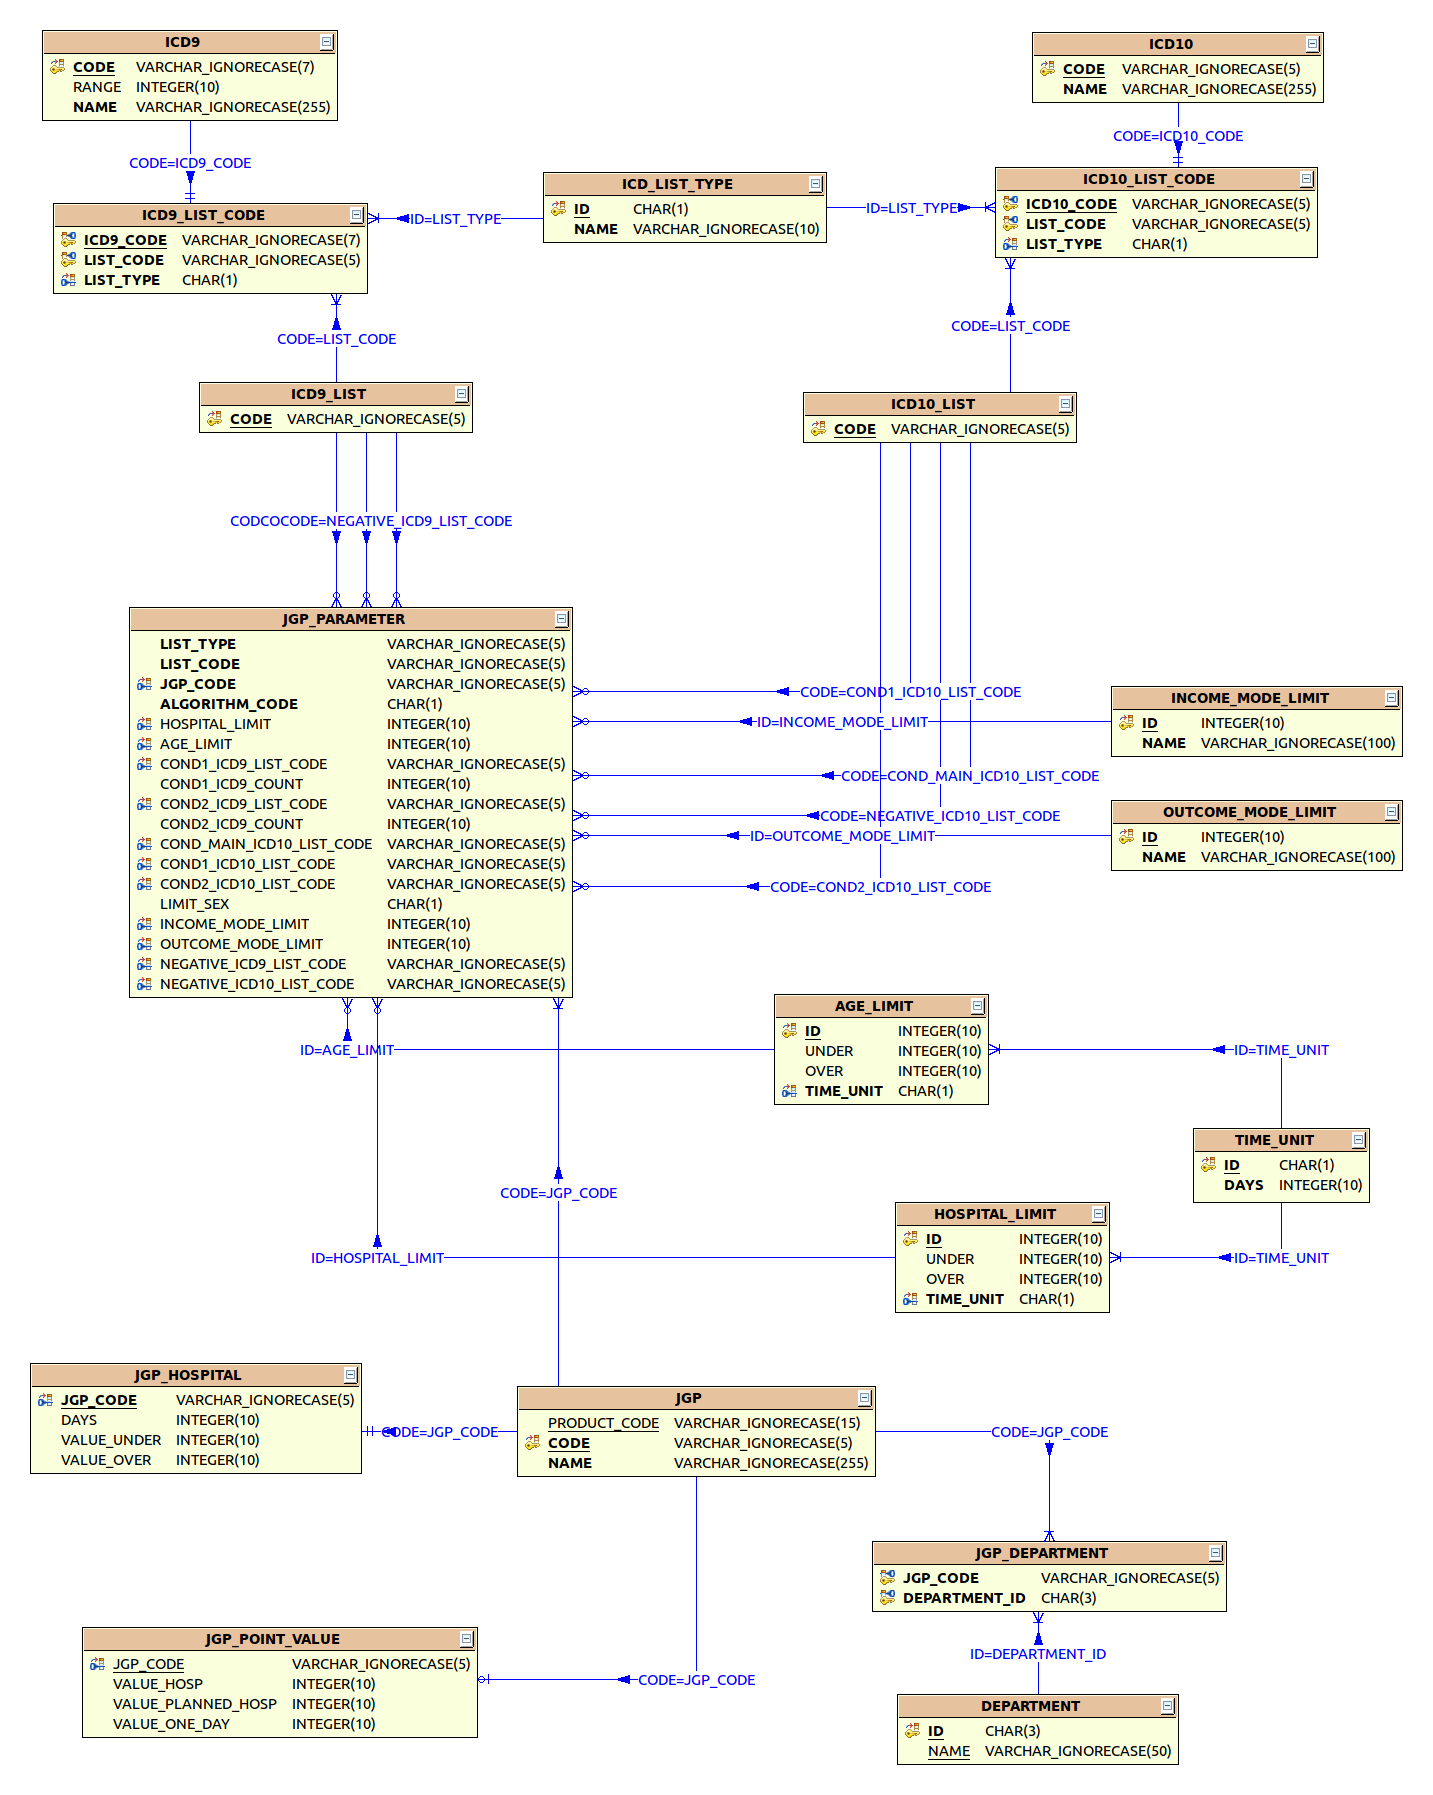
\includegraphics[scale=0.31]{images/erd}
\caption[Diagram ERD]{Diagram ERD. Autor: Mateusz Urbanik}
\label{img:diagram_erd}
\end{figure}

%---------------------------------------------------------------------------
%---------------------------------------------------------------------------
\section{Gruper NFZ}
\label{sec:gruperNFZ}

W tym podrozdziale znajduje się skrócony opis działania algorytmu ,,Grupera''. Kompletny opis algorytmu został przedstawiony w dokumencie ,,Informacje do przygotowania aplikacji grupera na potrzeby szpitalnych systemów informatycznych umożliwiającego kwalifikację rekordu pacjenta do właściwej grupy systemu Jednorodnych Grup Pacjentów'' opublikowanym przez NFZ\cite{algorytm_grupera}. Zawiera on słowny opis algorytmu oraz schematy blokowe, które są dalekie do standardów takich jak na przykład język UML. Należy w tym miejscu zaznaczyć, że specyfikacja udostępniona przez Fundusz jest jedynym źródłem wiedzy o zasadach kierujących algorytmem.
% Poznanie algorytmu grupera, zrozumienie zasad jakimi się on kieruje było kluczowym punktem pracy.

%---------------------------------------------------------------------------
\subsection{Zasady i logika grupowania}
\label{sec:zasadyLogikaGrupowania}
Wynikiem działania algorytmu ,,Grupera'' jest grupa JGP, która spełnia określony zestaw warunków. Lista grup JGP oraz zestaw warunków jest wyznaczany na podstawie danych wejściowych opisujących hospitalizację pacjetna. Algorytm w pierwszym kroku(w dużym uproszczeniu) wyznacza grupy JGP dla danych epizodu. Po wyznaczeniu listy grup następuje badanie tzw. mechanizmem przeliczania. Jeśli dana grupa zostanie zakwalifikowana do zmiany wartości punktowej zostaje ona zmieniona zgodnie z algorytmem mechanizmu przeliczania\cite{algorytm_grupera}. Diagram aktywności zilustrowany na rysunku \ref{img:diagram_activity_gruper} przedstawia działanie algorytmu ,,Grupera''.

\begin{figure}[!ht]
\centering
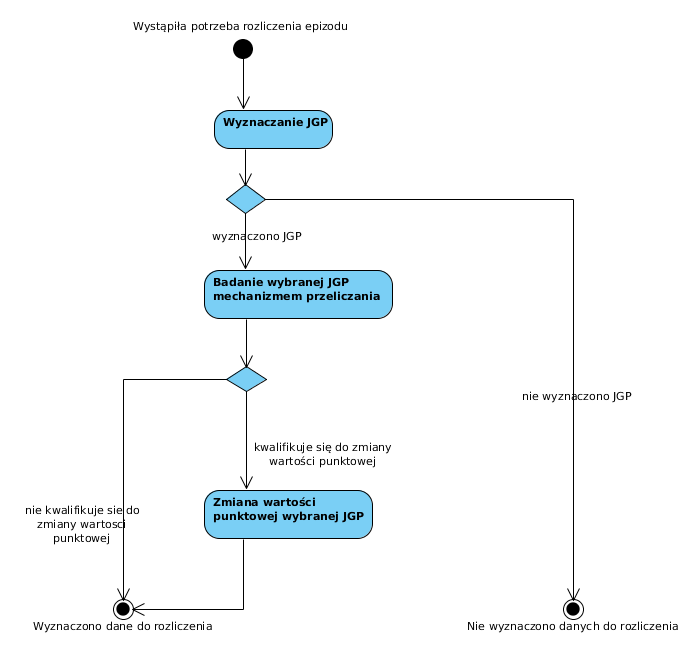
\includegraphics[scale=0.4]{images/activity-gruper}
\caption[Diagram aktywności]{Diagram aktywności - algorytm ,,Grupera''. Autor: Mateusz Urbanik}
\label{img:diagram_activity_gruper}
\end{figure}

%---------------------------------------------------------------------------
\newpage
\subsection{Proces wyznaczania grupy systemu JGP}
\label{sec:procesWyznaczaniaGrupySystemuJGP}
Proces wyznaczania grupy można podzielić na dwie główne gałęzie. Pierwsza gałąź(tzw. ścieżka 'ICD-9') wyznacza zbiór zakwalifikowanych grup wraz z warunkami do sprawdzenia na podstawie procedur znaczących. Druga ścieżka 'ICD-10' wyznacza analogicznie zbiór zakwalifikowanych grup, ale na podstawie rozpoznań zasadniczych. Ścieżka dla rozpoznań jest wybierana przez program jeśli spełniony jest jeden z następujących warunków:
\begin{itemize}\itemsep2pt
\item w danych epizodu nie występuje żadna procedura
\item ranga procedury <= 2 i czas hospitalizacji > 1 dnia
\end{itemize}
Jeśli wymienione wyżej warunki nie są spełnione wybierana jest ścieżka ICD-9\cite{algorytm_grupera}.

Po wybraniu ścieżki wyznaczana jest lista kodów JGP wraz z zestawem warunków do przetestowania. Każda grupa, która spełnia wszystkie warunki jest zapisywana na liście wybranych grup. Proces wyznaczania grupy ilustruje diagram aktywnyści przedstawiony na rysunku~\ref{img:diagram_activity_jgp}.
\newpage
\begin{figure}[!ht]
\centering
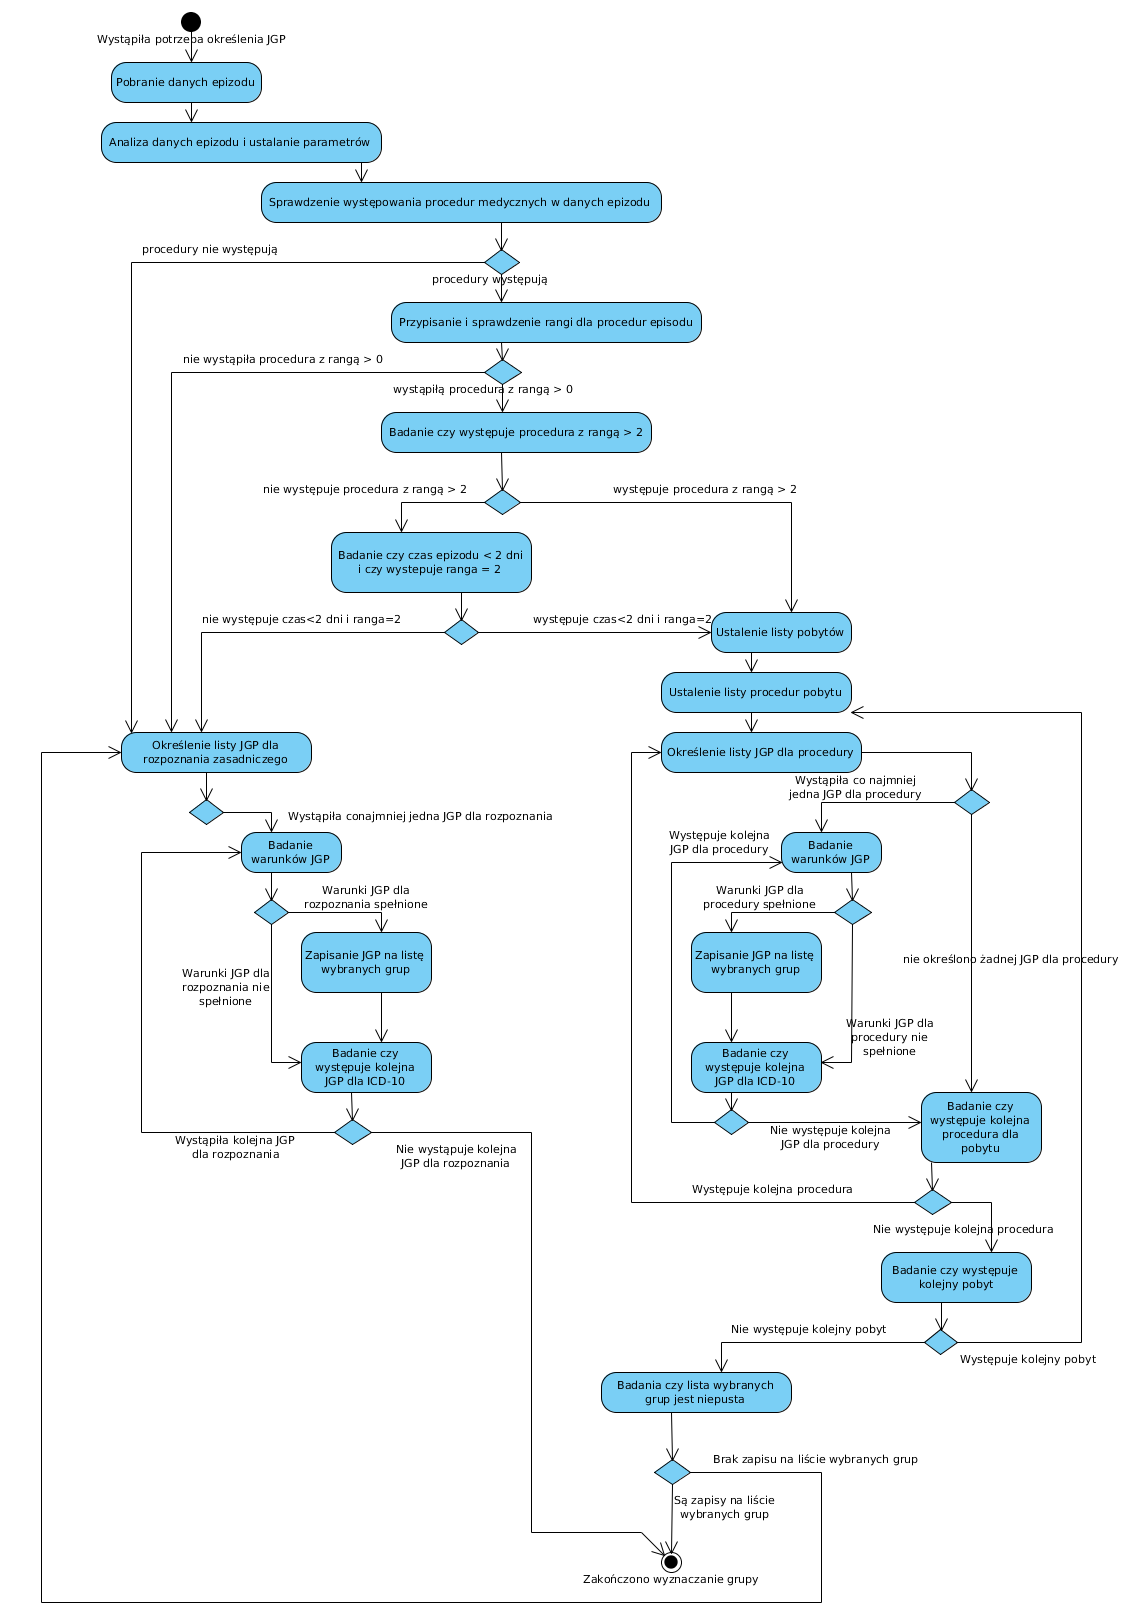
\includegraphics[scale=0.4]{images/activity-jgp} 
\caption[Diagram aktywności]{Diagram aktywności - wyznaczanie grupy JGP. Autor: Mateusz Urbanik}
\label{img:diagram_activity_jgp}
\end{figure}

%---------------------------------------------------------------------------
\subsection{Warunki kierunkowe}
\label{sec:warunkiKierunkowe}
Warunki kierunkowe są to wymagania decydujące o przebiegu grupowania. Każdy z warunków został oznaczony literą alfabetu. Ich dokładny opis znajduje się w dokumencie NFZ definiującym algorytm grupera\cite{algorytm_grupera}. Procedura badająca warunki JGP w pierwszej kolejności sprawdza czy spełnione są warunki kierunkowe, ponieważ mają one największy wpływ na proces grupowania.

Sposób w jaki zdecydowano się zaimplementować warunki kierunkowe przedstawiają poniższe założenia:
\begin{itemize}
\item Każdy z warunków zapisany jest w bazie pojedynczą literą alfabetu (A-Z).
\item Każda z liter alfabetu zostanie zmapowana na odpowiednią wartość enuma 'Condition', który zawiera wszystkie sygnatury warunków kierunkowych.
\item Zdefiniowanych zostało 26 klas nazwanych dużymi literami alfabetu rozszerzających bazową klasę AbstractChecker oraz implementujących metodę \mbox{\textit{public abstract boolean checkCondition(Stay stay, JGPParameter parameter, List<Reason> reasons);}}
\item Utworzona została enum-mapa, w której kluczem jest wartość enum(sygnatura warunku kierunkowego), a wartością obiekt(singleton) przypisanego do niej 'sprawdzacza' warunków.
\end{itemize}
Zaletą takiego rozwiązania jest możliwość implementacji generycznego silnika do sprawdzania warunków kierunkowych. Zdefiniowano zatem algorytm działania takiego silnika. Dla każdego wybranego obiektu klasy \mbox{JGPParameter}(warunki które mają zostać sprawdzone) na podstawie odczytanej sygnatury warunku kierunkowego zostaje uruchamiany odpowiedni kawałek kodu JAVY sprawdzający poprawność warunków dla pobytu. Listing \ref{java_check} przedstawia kawałek kodu JAVY realizujący tą funkcjonalność.

\begin{lstlisting}[language=Java,caption={Metoda sprawdzająca warunki kierunkowe. Autor: Mateusz Urbanik},label=java_check]
private boolean checkDirectional(Stay stay, JGPParameter parameter, List<Reason> reasons) {
  //pobranie sygnatury(A-Z) warunku ktory powinien zostac sprawdzony
  Condition condition = parameter.getCondition();
  //pobranie checkera dla warunku z mapy
  AbstractChecker checker = conditionsMap.get(condition);
  Assert.notNull(checker, "not implemented checker for condition: " + condition);
  //uruchomienie odpowiedniego checkera i zwrocenie wyniku badania warunku
  return checker.checkCondition(stay, parameter, reasons);
}
\end{lstlisting}

Rozwiązanie to pozwoliło na zapis skomplikowanych warunków w bazie danych. Jednak zapisywanie sygnatury obiektu 'sprawdzacza warunków', sprawia że nadal ważna część logiki jest zapisana w kodzie. O rozwinięciu tego rozwiązania  i o sposobie zapisu całej logiki ,,checkera'' do bazy danych napisano więcej w rozdziale \ref{sec:systemEkspertowy}.

%---------------------------------------------------------------------------
\subsection{Mechanizm osobodni}
\label{sec:mechanizmOsobodni}
Wyznacznikiem kosztów leczenia pacjenta nie może być tylko wartość punktowa wyliczona na podstawie przypisanej do pacjenta grupy systemu JGP. Ważnym czynnikiem generującym koszty leczenia jest czas pobytu w szpitalu. Pożywienie, wymiana pościeli, podawane leki i inne koszty generowane są przez pacjenta w każdym dniu jego pobytu na oddziale. Dlatego do algorytmu ,,Grupera'' musiał zostać wprowadzony mechanizm osobodni\cite{szkoleniaJGP}. Na początku algorytm bada czy można zastosować mechanizm przeliczania, co obrazuje diagram aktywności \ref{img:diagram_activity_maday}.

\begin{figure}[!ht]
\centering
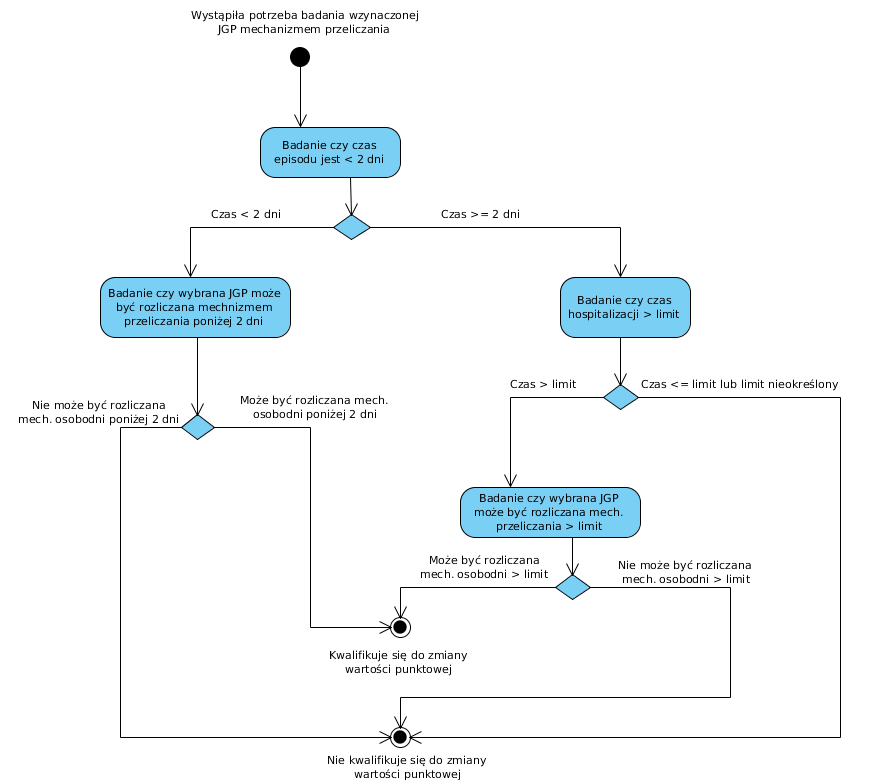
\includegraphics[scale=0.5]{images/activity-manday}
\caption[Diagram aktywności]{Diagram aktywności - mechanizm osobodni. Autor: Mateusz Urbanik}
\label{img:diagram_activity_maday}
\end{figure}

Jeśli wyznaczona grupa JGP dla epizodu nie kwalifikuje się do zmiany punktowej, pozostawiamy wartość wyznaczoną przez algorytm bez zmian. Natomiast jeśli zachodzi potrzeba zmiany wartości punktowej stosujemy następujący algorytm dla 2 przypadków:
\begin{itemize}
\item Jeśli czas hospitalizacji jest mniejszy od 2 dni ustalamy nową wartość punktową ustalaną na podstawie wartości 'poniżej 2 dni' z obiektu klasy JGPHospital. Należy zaznaczyć, że z powyższego mechanizmu są wyłączone zgony, świadczenia rozliczane w ramach umów z zakresu ,,zespół opieki dziennej'' oraz ,,zespół chirurgii jednego dnia''.
\item Jeśli czas trwania episodu jest większy lub równy 2 dni i jest większy od limitu ustalonego na podstawie wartości ,,dni'' z obiektu klasy JGPHospital. To wartość JGP jest ustalana poprzez powiększenie aktualnej wartości JGP o wynik iloczynu dni powyżej limitu z wartością punktową określoną przez wartość "powyżej".

NOWA WARTOŚĆ PUNKTOWA = STARA WARTOŚĆ + RÓŻNICA DNI PONAD LIMIT * WARTOŚĆ Z KOLUMNY ,,POWYŻEJ LIMITU''
\end{itemize} 

%---------------------------------------------------------------------------
%---------------------------------------------------------------------------
\section{System ekspertowy}
\label{sec:systemEkspertowy}

Stworzenie systemu ekspertowego jest zadaniem trudnym\cite{mulawka_ekspertowe}. Zdecydowano się na podejście ewolucyjne, w którym system w trakcie rozwijania go będzie dążył do rozwiązania spełniającego założenia systemu ekspertowego. Zbliżanie się w kierunku systemu ekspertowego oznacza, że nie powstaje on od razu, ale w wyniku przekształceń pewnych części systemu. Zmiany zachodzące w implementacji sprawiają, że staje się ona coraz bardziej generyczna i uniwersalna. Zaletą takiego podejścia jest powolne, jasne i zrozumiałe wprowadzanie zmian w kodzie źrodłowym systemu, w trakcie których system ciągle spełnia stawiane mu wymagania. Wadą jest potrzeba dużego nakładu pracy, aby uzyskać w efekcie generyczny system ekspertowy\cite{zielonogorski_ekspertowe}.

\subsection{Klasyfikacja}
\label{sec:klasyfikacjaSystemuEkspertowego}
W tym podrozdziale zakwalifikowano stworzony system do odpowiednich klas systemów ekspertowych:
\begin{itemize}
 \item Ze względu na możliwość ingerencji człowieka w produkowane przez system rozwiązanie jest to tzw. system doradczy \textendash{} podpowiada rozwiązanie pomagając podjąć decyzję użytkownikowi \textendash{} prezentuje rozwiązanie jakiegoś problemu, ale do użytkownika należy jego ocena, oraz to czy je zaakceptuje, czy odrzuci\cite{goluchowski_eskpertowe}.
 \item Ze względu na złożoność jest to system płytki - tzn. taki który korzysta tylko z informacji zgromadzonych w bazie wiedzy\cite{goluchowski_eskpertowe}.
 \item Ze względu na dane otrzymywane na wyjściu\cite{mulawka_ekspertowe} jest to system:
   \begin{itemize}
    \item Diagnozy \textendash{} ocena istniejącego stanu na podstawie posiadanych danych,
    \item Planowania \textendash{} opis stanu, do którego należy dążyć.
   \end{itemize}
 \item Ze względu na rodzaj przetwarzanej informacji jest to system z wiedzą pewną\cite{mulawka_ekspertowe}.
\end{itemize}

\subsection{Baza wiedzy}
\label{sec:bazaWiedzy}
Najważniejszym z punktu widzenia systemu ekspertowego jest podział wiedzy na bazę faktów oraz bazę reguł\cite{zielonogorski_ekspertowe}. Logiczne wyróżnienie faktów dla systemu grupera JGP, pozwoli spojrzeć na aplikację ,,Grupera'' jak na system ekpertowy. Wyróżniono zatem fakty: rekord pacjenta, płeć, oddział, rozpoznanie(ICD-10), procedura(ICD-9), tryb przyjęcia, tryb wypisu, Jednorodna Grupa Pacjentów, wartości punktowe dla JGP, czas hospitalizacji.

Zdefiniowano nastepujące warunki: warunki kierunkowe, warunek na rozpoznanie główne, warunek na rozpoznanie dodatkowe, warunek na procedurę zasadniczą, warunki na procedury dodakowe, warunek na procedury i rozpoznania wykluczające się, ograniczenie na czas hospitalizacji, ograniczenie na wiek.
Spełnienie wyżej wymienionych warunków powoduje wykonanie akcji: zapisanie kodu JGP na listę wybranych kodów. Reguła ta stosowana jest do wyznaczania listy zaakceptowanych grup JGP.

Proces wyznaczania nowych wartości mechanizmem osobodni, gdzie sprawdzane są warunki na czas hospitalizacji, a w przypadku ich spełnienia wyznaczana jest nowa wartość punktowa jest kolejnym przykładem reguły w systemie ekspertowym.

\subsection{Maszyna wnioskująca}
\label{sec:maszynaWnioskujaca}
Realizacja maszyny wnioskującej w języku JAVA odbywa się na poziomie warstwy biznesowej w technologii Spring. Klasa serwisowa przeprowadzająca proces wnioskowania zgodnie z wymaganiami systemu JGP to JGPService:

\begin{lstlisting}[language=Java,caption={Deklaracja interfejsu serwisu JGP. Autor: Mateusz Urbanik},label=java_jgp_service]
public interface JGPService {
    public List<JGP> findJGP(final JGPFilter filter);

    public JGPGroupResult group(Episode episode);

    public JGPGroupResult doByProcedures(Episode episode);

    public JGPGroupResult doByRecognitions(Episode episode);

    public void resolveResultsByJGP(Stay stay, List<JGPParameter> parameters, JGPGroupResult jgpGroupResult);

    public void recountManDay(Episode episode, List<JGPResult> jgpResultList);
}
\end{lstlisting}

Metoda ,,group'' sprawdza, którą ścieżkę wnioskowania obiera system. Istnieją dwie opcje: według rozpoznania głównego lub według procedur zasadniczych. Metody ,,doByRecognitions'' oraz ,,doByProcedures'' wyznaczają zbiór warunków z charakterystyki JGP do przeanalizowania. metoda ,,resolveResultsByJGP'' wykonuje zasadnicze wnioskowanie:
\begin{itemize}\itemsep1pt
 \item Sprawdza warunki określone w obiekcie klasy JGPParameter i jeśli zostaną zaakceptowane zapisuje je na liście accepted.
 \item Metoda sprawdza warunki kierunkowe, warunek na płeć, warunek na tryb przyjęcia i wypisu, warunek na leczenie w danym oddziale, warunki na współisteniejące i zasadnicze kody ICD , warunki na kody ICD wykluczające się(negatywne).
\end{itemize}

Podusmowując maszyna wnioskująca ma za zadanie poszukiwanie optymalnej grupy JGP. Realizuje ona proces wnioskowania w następujących krokach. Przyjmuje zbiór faktów wejściowych w postaci obiektu klasy Episode. Następnie wybiera ścieżkę(ICD9 lub ICD10) według której mają zostać ustalone parametry JGP. Po ustaleniu ścieżki - wyciągane są z bazy reguły które mają zostać sprawdzone w postaci obiektu klasy JGPParameter. Następuje sprawdzenie warunków i w przypadku spełnienia wszystkich grupa zostaje zapisana na liście zaakceptowanych grup.


%---------------------------------------------------------------------------
%---------------------------------------------------------------------------
\section{Optymalizacja JGP}
\label{sec:optymalizacjaJGP}

W tym podrozdziale opisane zostanie zagadanienie optymalizacji kosztów leczenia pacjenta. W poprzednim podrozdziale ustaliliśmy, że maszyna wnioskująca wybiera zbiór parametrów do przetestowania. Następnie dla grup JGP spełniających warunki zapisuje je na liście ,,zaakceptowane''. W tym miejscu nasunęły się pytania: A może by tak spróbować zapisać grupy JGP, które były testowane a zostały odrzucone przez algorytm na listę grup niezaakceptowanych? Może dla każdej niezaakceptowanej grupy JGP obliczyć jaką wartość punktową mogłaby przyjąć gdyby była zaliczona? Dlaczego została ona niezaakceptowana, jakich warunków nie spełniła? Może trzeba dla każdej niezaakceptwanej grupy zapisać na liście powód jej odrzucenia? 

Aby odpowiedzieć na powyższe pytania należy rozwinąć istniejący algorytm. Do obiektu klasy JGPResult dodałem listę niezaakceptowanych grup. Każda niezaakceptwana grupa będzie posiadać dodatkowo listę powodów niezaakceptowania - lista obiektów klasy Reason. W ten sposób, system będzie wiedział jakie warunki były testowane dla konkretnego rozwiązania oraz dlaczego nie zostały one zaakceptowane. 
Stworzyłem hierarchię klas dla powodów niezaakcpetowania:
\vspace*{0.2cm}
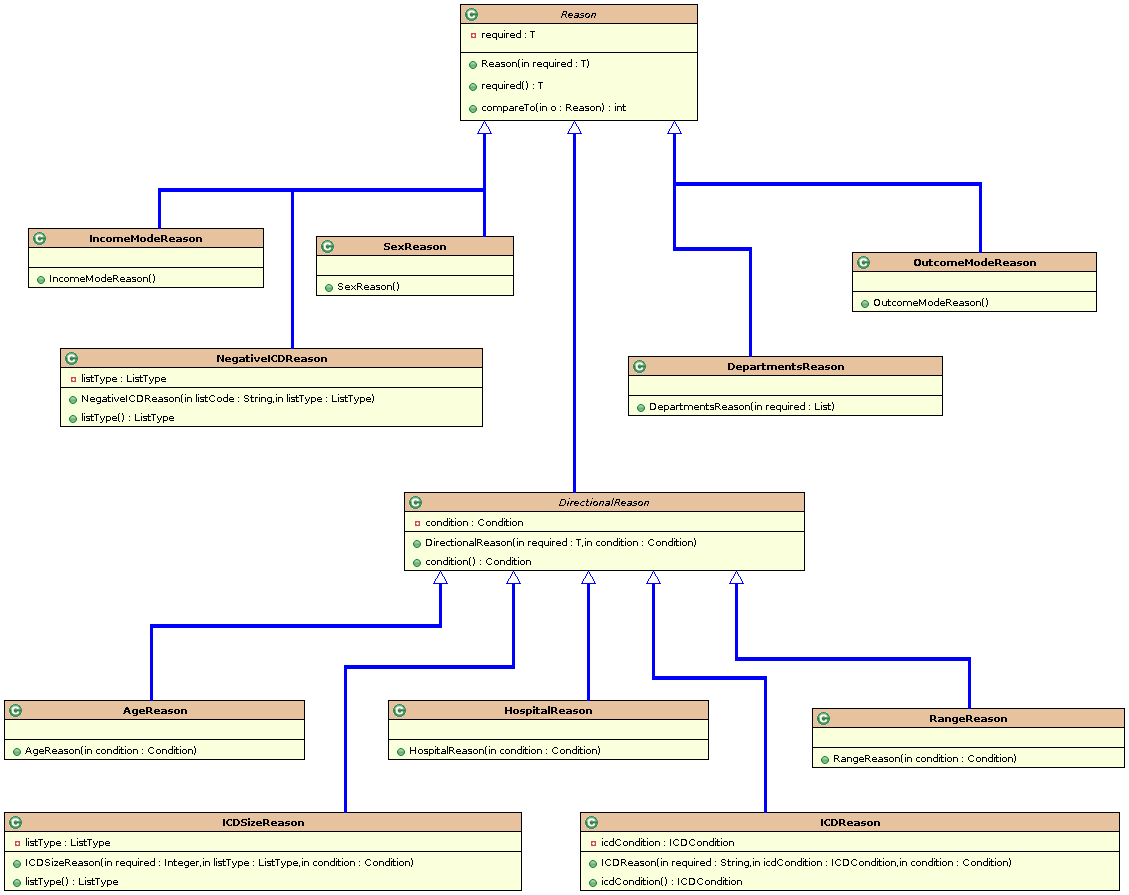
\includegraphics[scale=0.4]{images/reason-classes2}
\vspace*{0.2cm}
Rozszerzyłem listę argumentów każdej z metod checkerów o argument: lista powodów niezaakceptowania: List<Reason> reasons. 
Po sprawdzeniu konkretnego warunku, w przypadku jego niezaakceptowania tworzona jest odpowiednia instancja obiektu Reason, a następnie jest ona  dodawana do listy. Oto przykładowy kod:
\newpage
\begin{lstlisting}[language=Java]
protected boolean checkHospitalLimit(Stay stay, HospitalLimit hospLimit, List<Reason> reasons) {
     if (hospLimit != null) {
         int time = stay.getEpisode().hospitalTime(hospLimit.getTimeUnit());
         boolean result = hospLimit.test(time);
         if (!result) {
             reasons.add(new HospitalReason(hospLimit, condition()));
         }
         return result;
     }
     return true;
}
\end{lstlisting}

Metoda ,,checkHospitalLimit'' realizuje dopisanie powodu niezaakcpetowania grupy JGP w przypadku, gdy nie zostaje on zaakceptowany po wykonaniu testu. Powodem niezaakceptowania grupy systemu JGP może być niespełnienie warunku. Na przykład: czas hospitalizacji dla grupy JGP musi być większy niż 7 dni, a zdefiniowany czas leczenia jest równy 5 dni.

Takie podejście pozwala na stworzenie funkocjonalności, która będzie podpowiadać lekarzowi jakie może uzyskać grupy JGP z większą wartości punktową, czyli jak zmaksymalizować koszty leczenia pacjenta. Program podpowiadałby również jakie konkretnie warunki musi spełnić hospitalizacja, aby zaliczyć ją do droższej grupy (wybranej przez lekarza).

Zaimplementowanie mechanizmu ,,Reasons - powody niezaakceptowania do grupy'' odpowiada w systemie ekspertowym modułowi objaśniająco-wyjąśniającemu(ang. Explanation Facility). Jest to część systemu odpowiedzialna za wyprowadzanie na zewnątrz wniosków systemu. Moduł ten daje użytkownikowi radę, sugestię, ale nie podejmuje decyzji. Zwróćmy uwagę, że zapis historii niespełnionych warunków pozwala odtworzyć część ścieżki poszukiwania rozwiązania dla rozwiązań niespełniających warunków.
